\scanpage{248}
\margin{B) \uline{Case of punctured surfaces}}
\deleted{\unsure{In short.}}

That said, let us return to the situation of (53), of a topological space $X$, and of an $x\in X$ such that $X$ is a surface at $x$. Then the category \deleted{of \unsure{coverings}}
\[
\underline{\mathrm{Rev}}(D_x^*)
\]
is a Galois category, \inserted{abelian,} whose fundamental group is identified \unsure{canonically} with the orientation module $\overline T_x$ of $X$ at $x$
\[
(56)\qquad \pi_1(D_x^*)\overset{\mathrm{def}}=\pi_1(\underline{\mathrm{Rev}}(D_x^*))\simeq\overline T_x.
\]
This comes from the fact that the germ $D_x^*$ \deleted{\unsure{is} \illegible{1}} \inserted{admits a ``basis''} formed of spaces $D_{x,i}^*$ \deleted{\unsure{isomorphic to}} \inserted{\unsure{arising}} from the \uline{disks} with center $x$, and the $\pi_1$ of the said disks \unsure{form} a constant projective system\ldots

Thus the universal coverings $D_x^{*\sim}$ of $D_x^*$ form a connected groupoid, with fundamental \unsure{groupoid|group} $\deleted{\unsure{\mathbb{Z}}}\,\overline T_x$.

Let us therefore choose such a $D_x^{*\sim}$, and consider the composite morphisms

\scanpage{249}
\mspage{772}
\diagram{\begin{tikzcd}
D_x^{*\sim}\arrow[r] & D_x^*\arrow[r,hook] & X-\{x\}
\end{tikzcd}}
- more generally, let $S$ be a subset of $X$, containing $x$ as an isolated point (for example a discrete subset of $X$), so that we have
\diagram{\begin{tikzcd}
(57)\qquad D_x^*\arrow[r,hook] & U\overset{\mathrm{def}}=X\setminus S
\end{tikzcd}}
and consider the composites
\diagram{\begin{tikzcd}
(58)\qquad D_x^{*\sim}\arrow[r] & D_x^*\arrow[r,hook] & U.
\end{tikzcd}}
If $\underline{\mathrm{Rev}}(U)$ is \unsure{multi-Galois} (for example $U$ \inserted{locally} $\unsure{1|0}$-connected), then we can therefore consider the corresponding fundamental group of $U$
\[
(59)\qquad \pi_1(U,D_x^{*\sim}),
\]
I am going to define a \uline{canonical} \uline{homomorphism}
\diagram{\begin{tikzcd}[column sep=large]
(60)\qquad \unsure{K_x|\kappa_x}:\overline T_x\arrow[r] &
\underbrace{\pi_1(U,D_x^{*\sim})}_{\inserted{\begin{gathered}
\simeq\operatorname{Aut}\text{ of the fiber}\\
\text{functor }\underline{\mathrm{Rev}}(U)\longrightarrow\underline{\mathrm{Rev}}(D_x^{*\sim})\\
\text{on }\underline{\mathrm{Rev}}(U)
\end{gathered}}},
\end{tikzcd}}
we can describe it for example as
\diagram{\begin{tikzcd}
(61)\qquad \pi_1(D_x^*,D_x^{*\sim})\arrow[r]\arrow[d,phantom,"\simeq" description,sloped] & \pi_1(U,D_x^{*\sim})\\
\overline T_x &
\end{tikzcd}}

\scanpage{250}
induced by the inclusion
\diagram{\begin{tikzcd}
D_x^*\arrow[r,hook] & U
\end{tikzcd}}
or again, \deleted{\unsure{by}} in terms of \unsure{automorphisms} of a fiber functor, as the \deleted{\unsure{homomorphism}}operation of $\overline T_x$ on
\[
\Gamma\bigl(D_x^{*\sim},\underbrace{U'\mathbin{\times}_{\deleted{\unsure{D}}U}D_x^{*\sim}}_{\inserted{U'_{D_x^{*\sim}}}}\bigr)
\]
coming from the operations of $\overline T_x$ on $D_x^{*\sim}$.
\diagram{\begin{tikzcd}[column sep=small,row sep=small]
& U'_{D_x^{*\sim}}\arrow[dl]\arrow[dr] &\\
D_x^{*\sim}\arrow[dr] && U'\arrow[dl]\\
& U &
\end{tikzcd}}
\deleted{\illegible{1} \uline{N.B.} \unsure{Each time}}

Suppose that we have already chosen \inserted{separately} a fundamental group \inserted{$\pi_1(U,\widetilde U)=\pi$} of $U$, by the choice of a base point, or, more \unsure{generally}, of a universal covering $\widetilde U$ of $U$.
To compare it with $\pi_1(U,\deleted{\unsure{S}}D_x^{*\sim})$, we shall therefore choose a ``path of \unsure{domination}'' from $D_x^{*\sim}/U$ \unsure{to|:} $\widetilde U/U$, i.e. an isomorphism
\diagram{\begin{tikzcd}
(62)\qquad \widetilde U\arrow[r,"\sim"] & \mathrm{Revuni}(U,D_x^{*\sim})
\end{tikzcd}}
(universal covering of $\deleted{\unsure{\widetilde U}}U$ defined by the fiber functor
\diagram{\begin{tikzcd}
& \underline{\mathrm{Rev}}(U)\arrow[r] & \underline{\mathrm{Rev}}(D_x^{*\sim})\\
\inserted{\unsure{U}}\arrow[ur,bend right] &&
\end{tikzcd}}
\margin{\uline{N.B.} if \deleted{\illegible{1}} $D_x^{*\sim}$ defined by a universal covering $D_{x,i}^{*\sim}$ of a \unsure{punctured} disk $D_{x,i}^*$, and if $\widetilde y\in D_{x,i}^{*\sim}$, $\widetilde z\in\widetilde U$, $y,z$ the images in $U$, then
\[
\deleted{\unsure{D}}\mathrm{Revuni}(U,D_x^{*\sim})\simeq\mathrm{Revuni}(U,y)
\]
and $\widetilde U=\mathrm{Revuni}(U,z)$ : the choice of (62) \unsure{is equivalent to} that of a \unsure{path} from $y$ to $z$ ($\unsure{U}$ \unsure{locally} \unsure{1-connected}).}

\scanpage{251}
\mspage{773}
(the indeterminacy is \unsure{modulo} an \deleted{\unsure{automorphism}} \inserted{element} \deleted{\unsure{inner}} of $\pi$, or of $\pi_1(U,D_x^{*\sim})$) which induces an isomorphism
\diagram{\begin{tikzcd}
(63)\qquad \unsure{\pi_z|\pi_s|\pi}=\pi_1(U,\widetilde U)\arrow[r,leftrightarrow,"\sim"] & \pi_1(U,D_x^{*\sim})
\end{tikzcd}}
(which is changed by an inner automorphism, when we \unsure{change|compose} (62) by an element of $\pi$).

Composing (63) and (60), we therefore find a homomorphism
\diagram{\begin{tikzcd}
(64)\qquad \overline T_x\arrow[r] & \pi=\pi_1(U,\widetilde U),
\end{tikzcd}}
which depends on the choice of (62) -- and which, independently of this choice, defines a well-determined \uline{outer} \uline{homomorphism} -- which is none other than the outer homomorphism
\diagram{\begin{tikzcd}
(65)\qquad \pi_1(D_x^*)\arrow[r]\arrow[d,phantom,"\simeq" description,sloped] & \pi_1(U)\arrow[d,phantom,"\simeq" description,sloped].\\
\overline T_x & \pi
\end{tikzcd}}

\margin{C) \uline{Relation with} \uline{germs of arcs} (\unsure{playing} the role \deleted{\unsure{origin}} of ``base \unsure{points|point}'')}
I am going to describe a convenient way of fixing a universal covering $D_x^{*\sim}$ of $D_x^*$, by a \uline{germ} \uline{of an arc of a curve} \inserted{\uline{of} $X$,} \uline{issuing}

\scanpage{252}
from $x$. In general, let $I=[0,1]$, and $[I]$ be the \unsure{residual} germ of $I$ at $0$. \deleted{If $X$ is a space} \inserted{This is obviously a \uline{1-connected} \uline{germ}.}

\margin{Rather than \uline{\unsure{parametrize}} by germs of \unsure{neighborhoods} of $0$ in $[0,1]$, it would be more convenient for what follows to define a germ of an arc of $X$ issuing from $x$ as a germ of a \unsure{subset} of $X$ at $x$, satisfying \unsure{certain} properties\ldots.}

If $X$ is a topological space and $x\in X$, we call a germ of an arc of a curve \deleted{of} $X$ issuing from $x$, the morphisms
\diagram{\begin{tikzcd}
(66)\qquad [I]\arrow[r,"\gamma"] & \unsure{\mathrm{germ\,rés}}_x(X)\overset{\mathrm{def}}=D_x^*
\end{tikzcd}}
from the germ $[I]$ into the \unsure{residual} germ \inserted{$D_{X,x}^*$} of $X$ at $x$. Such a germ is therefore described by a continuous map from an interval $[0,\varepsilon]$ ($0<\varepsilon\leq1$)
\diagram{\begin{tikzcd}
(67)\qquad [0,\varepsilon]\arrow[r,"{\varphi\,\deleted{\unsure{\gamma}}}"] & X
\end{tikzcd}}
such that we have
\[
(68)\qquad\left\{\begin{array}{l}
\varphi(0)=x\\
\varphi(t)\neq x\quad\text{if }t\in]0,\varepsilon]
\end{array}\right.\quad.
\]
In the case we are interested in ($X$ a surface in a neighborhood of $x$, hence $\underline{\mathrm{Rev}}(D_x^*)$ \deleted{\unsure{Galois}} \inserted{Galois} abelian with group $\overline T_x$), we can use this morphism to define a fiber functor on $D_x^*$
\diagram{\begin{tikzcd}
(69)\qquad \underline{\mathrm{Rev}}(D_x^*)\arrow[r] & \underline{\mathrm{Rev}}([I]) & (\mathrm{Ens})\arrow[l,"\sim"']
\end{tikzcd}}

\scanpage{253}
\mspage{774}

hence a universal covering
\[
\tag{70}
D_x^{*\sim}\overset{\mathrm{d\acute ef}}{=}
\mathrm{Rev\,uni}\bigl(D_x^*,([I],\varphi)\bigr).
\]

Of course, we shall have a factorization
\diagram{\begin{tikzcd}[column sep=large]
[I] \arrow[r] \arrow[rr,bend right=18,"\varphi"'] &
D_x^{*\sim} \arrow[r] & D_x^*\;( \arrow[r,hook] & U)
\end{tikzcd}}

so we have a \unsure{canonical isomorphism}
\[
\tag{71}
\mathrm{Rev\,uni}(U,D_x^{*\sim})\simeq
\mathrm{Rev\,uni}(U,[I]),
\]
where $I$ is regarded as a $1$-connected germ over $U$ by the composite morphism
\diagram{\begin{tikzcd}
{[I]} \arrow[r] & D_x^* \arrow[r] & U.
\end{tikzcd}}

Thus we have
\diagram{\begin{tikzcd}[column sep=large]
{\text{(72)}\quad \pi_1(U,D_x^{*\sim})=\pi_1(U,[I])} &
\overline T_x. \arrow[l,"K_x"']
\end{tikzcd}}

\margin{D) \uline{Relation with differential structure}}
When $X$ is equipped with a differentiable structure in a neighborhood of $x$, we say that a germ of a curve in $X$ issuing from $x$ is \uline{differentiable}, if \unsure{the|the} \deleted{map}\inserted{germ} of a continuous map
\diagram{\begin{tikzcd}
I \arrow[r] & X
\end{tikzcd}}
which defines it is differentiable, \deleted{\unsure{Let us take|For this}}\inserted{and moreover}

\scanpage{254}

the tangent map at the origin, \deleted{\illegible{2} \unsure{leads to} a \unsure{morphism}}
\diagram{\begin{tikzcd}
{\text{(73)}\quad\mathbb R} \arrow[r] & \mathrm{Tang}_x(X),
\end{tikzcd}}
is injective. Then the image of $\mathbb R^+$ is a homogeneous half-line in the tangent space to $X$ at $x$, which we call the \uline{half-tangent} of the germ of an arc of a curve under consideration at $x$.

Returning for a moment to the purely topological case, we are going to consider the set $\unsure{\mathrm{Germarc}|\mathrm{Courarc}}(X,x)$ of germs of arcs of $X$ issuing from $x$, as the set of objects of a groupoid (the local fundamental groupoid of $X$ at $x$), taking as morphisms from $\gamma$ to $\gamma'$ \deleted{\unsure{a|the}} the isomorphisms from \deleted{$\mathrm{Rev\,uni}(D_x^*,\gamma)$} $D_{x,\gamma}^{*\sim}$ to $D_{x,\gamma'}^{*\sim}$
\[
\tag{74}
\mathrm{Isom}(\gamma,\gamma')\overset{\mathrm{d\acute ef}}{=}
\mathrm{Isom}_{D_x^*}(D_{x\gamma}^{*\sim},D_{x,\gamma'}^{*\sim}).
\]
We thus find \inserted{by construction} an equivalence of \deleted{categories (of} connected groupoids
\diagram{\begin{tikzcd}[column sep=large]
{\text{(75)}\quad\uline{\unsure{\mathrm{Germarc}|\mathrm{Courarc}}}(X,x)} \arrow[r] &
\uline{\mathrm{Rev\,uni}}(D_x^*).
\end{tikzcd}}

\scanpage{255}
\mspage{775}

Let on the other hand, in the case where $X$ is differentiable at $x$, \deleted{\unsure{Germ}}
\[
\tag{76}
\uline{\unsure{\mathrm{Germarc\,diff}|\mathrm{Courarc\,diff}}}(X,x)
\]
be the full subcategory of \deleted{$\unsure{\mathcal C_x|\mathcal G_x}$} $\uline{\unsure{\mathrm{Germarc}|\mathrm{Courarc}}}(X,x)$ formed by the differentiable germs of arcs. Let $\mathbb S_x$ \inserted{$\simeq\mathbb S^1$} be \deleted{the category}\inserted{the }space of half-lines of the Tangent space $\mathrm{Tang}_x(X)$
\[
\tag{77}
\mathbb S_x=
\begin{array}{l}
\inserted{\text{space of}}\\
\text{Half-lines}\\
\text{of }\mathrm{Tang}_x(X)
\end{array}
\simeq\mathbb S^1,
\]
and let us consider the fundamental groupoid
\diagram{\begin{tikzcd}[column sep=large]
{\text{(78)}\quad\Pi_1(\mathbb S_x)} \arrow[r,"\approx"] & \uline{\mathrm{Rev\,uni}}(\mathbb S_x).
\end{tikzcd}}

\margin{\figure{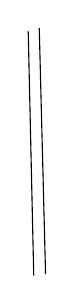
\begin{tikzpicture}[x=1cm,y=1cm]
\draw (0,0) -- (0.07,-3.1);
\draw (0.14,0.04) -- (0.22,-3.08);
\end{tikzpicture}}}
I am going to define an equivalence of categories
\diagram{\begin{tikzcd}[column sep=large,row sep=large]
{\text{(79)}\quad\uline{\unsure{\mathrm{Germarc\,diff}|\mathrm{Courarc\,diff}}}(X,x)} \arrow[r,"\approx"] \arrow[d,"\approx"{rotate=90}] &
\Pi_1(\mathbb S_x) \arrow[d,"\approx"{rotate=90}]\\
\uline{\mathrm{Rev\,uni}}(D_x^*) & \uline{\mathrm{Rev\,uni}}(\mathbb S_x)
\end{tikzcd}}
which, on the sets of objects, is to be the map \unsure{associating} to $\forall$ differentiable germ of an arc at $x$ its half-\uline{tangent}. The question is thus, if $\gamma,\gamma'$ are two such arcs, corresponding to half-tangents $\Delta,\Delta'$, to define a canonical bijection


\scanpage{256}

\margin{\figure{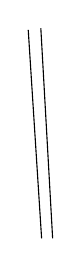
\begin{tikzpicture}[x=1cm,y=1cm]
\draw (0,0) -- (0.17,-2.65);
\draw (0.16,0.02) -- (0.31,-2.65);
\end{tikzpicture}}}
\diagram{\begin{tikzcd}[column sep=huge,row sep=large]
{\text{(80)}\quad\mathrm{Isom}(\gamma,\gamma')} \arrow[r,"\sim"] \arrow[d,equal,"\mathrm{d\acute ef}"] &
\mathrm{Isom}_{\Pi_1\mathbb S_x}(\Delta,\Delta') \arrow[d,equal,"\mathrm{d\acute ef}"]\\
\mathrm{Isom}(D_{x,\gamma}^{*\sim},D_{x,\gamma'}^{*\sim}) &
{\begin{array}{l}
\text{classes of paths}\\
\text{in }\mathbb S_x^*\text{ from }\Delta\\
\text{to }\Delta'
\end{array}}
\end{tikzcd}}

\deleted{\illegible{1}}
Instead of defining the bijection (80) directly, I am going to define rather a functor (which will be an equivalence of categories)
\diagram{\begin{tikzcd}[column sep=large]
{\text{(81)}\quad\Theta:\Pi_1(\mathbb S_x)} \arrow[r,"{(\deleted{\unsure{\to|\sim}}\approx)}"] &
\uline{\mathrm{Rev\,uni}}(D_x^*),
\end{tikzcd}}

Let \deleted{$\mathcal A$}
\[
\tag{82}
\left\{
\begin{array}{l}
\mathcal A_x\text{ set of }\inserted{\text{closed}}\text{ }1\text{-connected subsets of }\mathbb S_x\\
(\text{i.e. }\uline{\text{arcs}}\text{ of a circle in }\mathbb S_x,\\
\quad\unsure{\text{possibly}}\text{ reduced }\unsure{\text{to}}\text{ points,}\\
\quad\text{but }\ne\mathbb S_x)
\end{array}
\right.
\]
this is an ordered set, \unsure{and one|thus} \deleted{the set} defines an ordered category $\uline{\mathcal A}_x$ (the objects are the $\in\mathcal A_x$, the arrows are the inclusions) --- and we know that the enveloping groupoid \inserted{$\uline{\mathrm{Gr}}(\uline{\mathcal A}_x)$} of this ordered category is canonically equivalent to $\Pi_1(\mathbb S_x)$,


\scanpage{257}
\mspage{776}

more precisely, let \deleted{$\unsure{\uline{\mathcal A}_{0x}|\uline{\mathcal A}_x}$}\inserted{$\uline{\mathrm{Gr}}_0(\uline{\mathcal A}_x)$} be the full subcategory of $\uline{\mathrm{Gr}}(\uline{\mathcal A}_x)$ (whose set of objects is $\mathcal A_x$) whose objects are the \uline{one-point} arcs, \& we then have a canonical equivalence
\diagram{\begin{tikzcd}[column sep=large]
{\text{(83)}\quad\uline{\mathrm{Gr}}_0(\uline{\mathcal A}_x)} \arrow[r,"\approx"] & \Pi_1(\mathbb S_x)
\end{tikzcd}}
which on objects reduces to $\{a\}\longmapsto a$, and which, for any arc \deleted{$\unsure{\mathbb S|\xi}$} $A$ with endpoints $a,b$, whence inclusion isomorphisms \unsure{in|in} $\uline{\mathrm{Gr}}(\mathcal A_x)$
\diagram{\begin{tikzcd}[column sep=normal,row sep=large]
{\text{(84)}\quad\raisebox{-1.6em}{$\left\{\rule{0pt}{3.2em}\right.$}} &
a \arrow[r,"\sim"] & A & b \arrow[l,"\sim"'] & \\
& \text{whence}\quad a \arrow[rr,"\sim"] & & b & \text{in }\uline{\mathrm{Gr}}(\mathcal A_x)
\end{tikzcd}}
associates to this arrow $a\overset{\sim}{\longrightarrow}b$ of $\uline{\mathrm{Gr}}_0(\mathcal A_x)$ the arrow of $\Pi_1(\mathbb S_x)$, defined by the arc $A$ regarded as a path from $a$ to $b$.

Thus, for $\forall$ groupoid $\mathcal G$, giving a functor
\diagram{\begin{tikzcd}[column sep=large]
{\text{(85)}\quad\Psi:\Pi_1(\mathbb S_x)} \arrow[r] & \mathcal G
\end{tikzcd}}
is equivalent to giving a functor

\scanpage{258}
\[
\tag{86}
\Psi : \underline{\mathcal A}_x \longrightarrow \mathcal G
\]
and (85) is an equivalence of categories iff
$\mathcal G$ is \deleted{\unsure{connected}} connected and
\deleted{\unsure{the}} its $\unsure{\pi_1|\Pi_1}$ is $\simeq\mathbb Z$, and if, for
\deleted{\unsure{an $x$ of}}\inserted{a pair $(a,b)$ of}
distinct points $a,b$ of $\unsure{\mathbb S_x}$, defining two arcs $A$ and $B$
with endpoints $a,b$, \deleted{of}considering the automorphism of $a$ in
$\underline{\mathrm{Gr}}_0(\mathcal A_x)$ i.e. in
$\underline{\mathrm{Gr}}(\mathcal A_x)$, composed of
\[
\tag{86bis}
\diagram{\begin{tikzcd}[column sep=small]
\{a\} \arrow[r,"\sim"] & A & \{b\} \arrow[l,"\sim"'] \arrow[r,"\sim"] & B & \{a\} \arrow[l,"\sim"']
\end{tikzcd}}
\]
the corresponding automorphism of $\Psi(\{a\})$ in $\mathcal G$
is a \uline{generator} of $\mathrm{Aut}_{\mathcal G}(\Psi(\{a\}))$.

We are thus going to define a functor
\[
\tag{87}
\underline{\mathcal A}_x \longrightarrow
\underline{\mathrm{Revuni}}(D_x^*)
\]
\deleted{and} (satisfying the additional condition stated).
To define such a functor, it suffices to define a functor
\[
\tag{88}
\underline{\mathcal A}_x \longrightarrow
\begin{gathered}
\text{category of 1-connected germs}\\
\text{of spaces, \unsure{over|over} the}\\
\text{germ }D_x^*
\end{gathered}
\]

\scanpage{259}
\mspage{777}
by composing this functor with the functor
\[
\tag{89}
\begin{gathered}
\text{category of 1-connected germs}\\
\text{of spaces \unsure{over|over}}\\
\text{the germ }D_x^*
\end{gathered}
\longrightarrow \underline{\mathrm{Revuni}}(D_x^*).
\]
In fact, (88) \unsure{will associate|we associate} to $\forall\ A\in
\deleted{\unsure{\mathcal E}}\mathcal A_x$ a
\deleted{germ of a \unsure{subspace} of $X$ at $x$, of which}
\inserted{filter on $X-x$ tending to $x$, of which}
we will take the germ \deleted{\unsure{residual}}.

\deleted{\unsure{The half-lines}}
\inserted{The elements \inserted{$A$} of}
$\mathcal A_x$ are obviously identified with the \uline{cones}
\deleted{\unsure{open}}\inserted{closed $C$}
in $\mathrm{Tang}_x(X)$, \deleted{\unsure{disti}}
distinct from $\{0\}$ and from the
\inserted{\unsure{tangent$^{\mathrm t}$|tangent}} space $\forall$ entire.
\deleted{\unsure{Let $C$ be a}}
\inserted{Let $\unsure{C\mathcal A_x|C\in\mathcal C\mathcal A_x}$ be one of these cones.}
Let us consider a local isomorphism
\deleted{\unsure{a}}
\[
\tag{90}
f:(\mathrm{Tang}_x(X),0)\deleted{\unsure{\&}}
\xrightarrow{\sim}(X,x),
\]
\deleted{whose map}
\inserted{whose map} on tangent spaces is the identity.
\deleted{When} If $C$ is a cone $\in\mathcal C\mathcal A_x$,
its image under such an isomorphism depends on the choice of the local isomorphism in question.
But let us consider the \deleted{\unsure{family|set of}}
\inserted{filter base}
\deleted{\unsure{arcs}}\inserted{of} cones
\inserted{$C'\in\mathcal C\mathcal A_x$} containing
\deleted{$\unsure{\in}$} $C$ \uline{strictly}
(i.e. corresponding to arcs $A'$ which are \uline{neighborhoods}
of $A$, or again such that $C'-\{0\}$ is a neighborhood of
$C\setminus\{0\}$), then the

\scanpage{260}
\deleted{germ of spaces defined by the base}
\inserted{the image under (90) \deleted{\unsure{of this}}
\inserted{of the filter defined by the} base of a}
filter on $\mathrm{Tang}_x(X)$ formed by the
$V\cap(C'\setminus\{0\})$ \unsure{, where|:} $V$
ranging over the neighborhoods of $0$ in $\mathrm{Tang}_x(X)$,
is a filter on $X\setminus\{x\}$ which no longer depends on the choice of $f$,
and which tends to $x$, hence defines a germ of spaces
\inserted{$\widetilde A$ or $\widetilde C$}
over \deleted{$\unsure{X_x|X}$} $D_x^*$.
This germ of spaces, \deleted{\unsure{is é|and it}}
isomorphic to the germ of spaces defined by $\mathrm{Tang}_x(X)$ endowed with the filter
with base the $V\cap(C'-\{0\})$ --- where one can take $V$
convex closed \unsure{symmetric|symmetric}, hence
$V\cap(C'-\{0\})$ contractible --- is obviously 1-connected.
For $A$ i.e. $C$ varying \unsure{i.e.} for $A_1\subset A_2$
i.e. $C_1\subset C_2$ we have the corresponding inclusion relation
\inserted{\deleted{$\unsure{A}$}
\diagram{\begin{tikzcd}
\widetilde C_1 \arrow[r] & \widetilde C_2
\end{tikzcd}}}
on the germs of spaces in $D_x^*$.
We thus do get (88), whence (87)\inserted{and (81)}, and we check
that the latter is indeed an equivalence of \deleted{categories}
groupoids, via the \unsure{verification|verification$^{\mathrm t}$}
\deleted{\unsure{by}} \unsure{made explicit|made explicit} above ((86bis)).

\scanpage{261}
\mspage{778}
Let us now consider, once again, a differentiable arc $\gamma$ in $X$
issuing from $x$, and its half-tangent $\Delta$.
Then $\{\Delta\}\in\mathcal A_x$, and we can consider the germ
of spaces $\{\Delta\}^{\sim}$ over $D_x^*$.
We have \inserted{\unsure{the|some}} two canonical inclusion morphisms
\[
\tag{91}
\diagram{\begin{tikzcd}
\gamma \arrow[r,hook] & \{\Delta\}^{\sim} \arrow[r,hook] & D_x^*
\end{tikzcd}}
\]
and we deduce from this a canonical isomorphism
\[
\tag{92}
\diagram{\begin{tikzcd}[column sep=large]
\mathrm{Revuni}(D_x^*,\gamma) \arrow[r,phantom,"\simeq"] \arrow[d,equal,"\mathrm{déf}"]
& \mathrm{Revuni}(D_x^*,\{\Delta\}^{\sim}) \arrow[d,equal,"\mathrm{déf}"] \\
D_{x,\gamma}^{*\sim} & \Theta(\Delta)
\end{tikzcd}}
\]
If $\gamma'$ is another differentiable arc at $x$, corresponding to the half-tangent
$\Delta'$, we thus have
\[
D_{x,\gamma}^{*\sim}\simeq\Theta(\Delta),\qquad
D_{x,\gamma'}^{*\sim}=\Theta(\Delta')
\]
whence
\[
\diagram{\begin{tikzcd}[column sep=large,row sep=large]
\mathrm{Isom}(D_{x,\gamma}^{\unsure{*}\sim}\unsure{\}},D_{x,\gamma'}^{*\sim})
\arrow[r,phantom,"\simeq"] \arrow[d,equal,"\mathrm{déf}"]
& \mathrm{Isom}(\Theta(\Delta),\Theta(\Delta')) \\
\mathrm{Isom}(\gamma,\gamma')
& \mathrm{Isom}_{\Pi_1(\mathbb S_x)}(\Delta,\Delta')
\arrow[u,"\sim","\Theta"']
\end{tikzcd}}
\]
which is the \deleted{\unsure{right}} bijection (80) sought.

\deleted{Let} In summary, we have an essentially commutative diagram of equivalences
of groupoids

\scanpage{262}
\[
\tag{93}
\diagram{\begin{tikzcd}[column sep=huge,row sep=huge]
\underline{\mathrm{germesdiff}}(X,x)
\arrow[r,"{\substack{\gamma\longrightarrow\underline\Delta(\gamma)\\\approx}}"]
\arrow[d,"\approx","{\substack{\gamma\mapsto\mathrm{Revuni}(D_x^*,\gamma)\\=D_{x,\gamma}^{*\sim}}}"']
& \Pi_1(\mathbb S_x)
\arrow[d,"{\approx\quad a\mapsto\mathrm{Revuni}(\mathbb S_x,\cdot)}"]
\arrow[dl,dashed,"{\Theta\ \approx}"'] \\
\underline{\mathrm{Rev.uni.}}(D_x^*) \arrow[r,"\approx"]
& \mathrm{Revuni.}(\mathbb S_x)
\end{tikzcd}}
\]
\margin{Of course, the difficulty here came from the fact that we had no
direct morphism between the germ $D_x^*$, and the space $\mathbb S_x$...}

\unsure{The} only functor that has not yet made explicit is the functor
\[
\tag{94}
\diagram{\begin{tikzcd}[column sep=small,row sep=small]
\underline{\mathrm{Revuni}}(D_x^*)
\arrow[rr,"\approx"] \arrow[dr,dashed,"{\Theta^{-1}}"']
& & \mathrm{Revuni}(\mathbb S_x) \\
& \Pi_1(\mathbb S_x) \arrow[ur,"{\mathrm{can}}"'] &
\end{tikzcd}}
\]
defined as the composite of $\Theta^{-1}$ with the canonical functor
$\Pi_1(\mathbb S_x)\longrightarrow\mathrm{Rev.uni.}(\mathbb S_x)$.

Finally, in these considerations of differential topological geometry,
the key construction is that of the functor $\Theta$ (81).
We have taken some pains to define it in an invariant way.
In the case where we have a local isomorphism
\[
\tag{90}
f:\bigl(\underbrace{\mathrm{Tang}_x(X)}_{V},0\bigr)\longrightarrow(X,x),
\]
the construction of \unsure{this|---} $\Theta$ can be made explicit as
a canonical construction in a vector space $V$.
Every homogeneous half-line

\scanpage{263}
\mspage{779}

$\Delta$ in $V$ defines a germ of arcs (\unsure{differentiable}) in $V$ issuing from $0$, whence a corresponding universal covering $D_{V,0;\Delta}^{*\sim}$ of $D_{V,0}^{*}$, hence a universal covering $D_{x,\Delta}^{*\sim}$ of $D_x^*$.
We must see how this $D_{x,\Delta}^{*\sim}$ depends ``continuously'' on $\Delta$, and what amounts to the same thing, how the universal covering $V_{\Delta}^{*\sim}$ of $V^*=V\setminus\{0\}$ depends continuously on $\Delta$, which is quite \unsure{standard}\unsure{...}.

Now let \inserted{$\unsure{u|\varphi}$} be \unsure{an} an \deleted{diffeomorphism}\inserted{\unsure{automorphism}} of $X$, fixing $x$, and differentiable at $x$. We thus have \deleted{\unsure{some}} \unsure{automorphisms} induced \deleted{of}
\[
\tag{\unsure{95|94}}
{}^{\unsure{u|\varphi}}D_x^*\quad\text{automorphism of }D_x^*,\qquad
{}^{\unsure{u|\varphi}}\mathbb S_x\quad\text{automorphism of }\mathbb S_x.
\]

Consider on the other hand a universal covering $\widetilde{\mathbb S}_x$ of $\mathbb S_x$, and let $D_x^{*\sim}$ be an associated universal covering of $D_x^*$, thanks to the equivalence (94). I say that we then have a

\scanpage{264}

canonical bijection
\[
\tag{96}
\diagram{\begin{array}{c@{\qquad}c@{\qquad}c}
\text{set of liftings}&\simeq&\text{set of liftings}\\
\text{of }{}^uD_x^*\text{ to an}&&\text{of }{}^u\mathbb S_x\text{ to an}\\
\text{automorphism }{}^uD_x^{*\sim}\text{ of the}&&\text{automorphism }{}^u\mathbb S_x^\sim\text{ of}\\
\text{germ }D_x^{*\sim}&&\mathbb S_x^\sim
\end{array}},
\]
\margin{the construction (96) will be carried out in the following pages, leading to (122) page \unsure{783}}
bijection which is an isomorphism of $\overline T_x$-torsors.
(where $\overline T_x$ is the $\mathbb Z$-orientation module of $X$ at $x$, let us recall).

\margin{E) \uline{Axiomatization} : \unsure{the structure|structure} of \uline{correlation} between universal coverings $\mathbb S_x^\sim$ \uline{and} $D_x^{*\sim}$.}
I feel like giving an axiomatic description of (94) and (96).

1) Let \inserted{$D_x=$} $(X,x)$ be a germ of a differentiable surface, whence
$V_{X,x}=V_x=\mathbb V=\operatorname{Tang}_x(X)$,
and $\mathbb S_x=V^*/\mathbb R^{*+}$ (where $\mathbb V^*=V\setminus\{0\}$), as well as $D_{X,x}^*=D_x^*$.
\margin{``germ'' : we \unsure{tacitly include} the filter of neighborhoods of $x$ in $X$}
\deleted{Let $\mathbb S_x^\sim$ (\unsure{resp.} $D_x^{*\sim}$) be \unsure{universal} coverings of $\mathbb S_x$ (resp. $D_x^*$).}
\inserted{We denote by}
\deleted{$\unsure{\mathcal A|\in}$}
$\mathcal A_{X,x}$ \unsure{or} $\mathcal A_x$ the set of \uline{arcs} of $\mathbb S_x$, in one-to-one correspondence with the set $\mathcal C_{X,x}=\mathcal C_x$ of
\deleted{``\unsure{angular sectors}'' of $V$ \unsure{proper}}
\inserted{``closed cones'' \unsure{proper}} of $V$ ($\ne V$ and $\{0\}$).
For $A\in\mathcal A_x$ or $C\in\mathcal C_x$, we denote by
\deleted{$\unsure{\widetilde A|f(A)}$ \unsure{or} $\unsure{\widetilde C|f(C)}$}
\inserted{$\unsure{\mathrm{Ep}|E_p}(A)$ or $\unsure{\mathrm{Ep}|E_p}(C)$}
the corresponding germ of spaces over $D_x^*$.
\margin{``\unsure{thickening}'' \deleted{\unsure{image|germ}} of $A$ (or of $C$) in $D_x^*$}
If $\widetilde{\mathbb S}$ is a universal covering of $\mathbb S$, $\widetilde D_x^*$ a universal covering of $\widetilde D_x^*$, we consider the sets

\scanpage{265}
\mspage{780}

\[
\tag{97}
\diagram{\begin{array}{r@{\,}c@{\qquad}c@{\qquad}r@{\,}c}
&\Gamma\bigl(\deleted{\unsure{\mathbb S|\widetilde A}}A,\mathbb S_x^\sim/\mathbb S_x\bigr)&,&
&\Gamma\bigl(\inserted{\unsure{\mathrm{Ep}|E_p}}(\widetilde A),D_x^{*\sim}/D_x^*\bigr)\\
&\Vert&&&\Vert\\
&\operatorname{Hom}_{\mathbb S}(A,\mathbb S_x^\sim)&&&\operatorname{Hom}_{D_x^*}(\widetilde A,D_x^{*\sim})\\
\mathrm{déf}&\Vert&&\mathrm{déf}&\Vert\\
&\mathbb S_x^\sim(A)&&&D_x^{*\sim}\bigl(\unsure{\mathrm{Ep}|E_p}(A)\bigr)
\end{array}}
\]
which are both Torsors under the same group $\overline T_{X,x}=\overline T_x$ (the $\mathbb Z$-module of orientations of $X$ at the point $x$). Consider the set
\[
\tag{98}
H(A)=\operatorname{Isom}_{\unsure{T_x|\overline T_x}}\bigl(\mathbb S_x^\sim(A),
\deleted{\unsure{D_x^{*\sim}(\widetilde A)}}\unsure{)}
\inserted{D_x^{*\sim}\bigl(\unsure{\mathrm{Ep}|E_p}(A)\bigr)}\bigr)
\]
which is itself a $\overline T_x$-torsor. If we have \deleted{\illegible{1}} an inclusion
\[
A\subset A'
\]
we deduce from it, by restriction, isomorphisms of $\overline T_x$-torsors
\[
\tag{99}
\mathbb S_x^\sim(A')\xrightarrow{\sim}\mathbb S_x^\sim(A),\qquad
D_x^{*\sim}\bigl(\unsure{\mathrm{Ep}|E_p}(A')\bigr)
\unsure{-|\longrightarrow}
D_x^{*\sim}\bigl(\unsure{\mathrm{Ep}|E_p}(A)\bigr)
\]
whence a canonical isomorphism
\[
\tag{100} H(A)\xrightarrow{\sim}H(A')
\]
so that \deleted{$A\unsure{\longmapsto|\longleftarrow}H(A)$ \unsure{defines}}
\[
\tag{101}
A\longmapsto H(A),\quad\text{functor}\quad
\underline{\mathcal A}_x\xrightarrow{H}\underline{\operatorname{Tors}}(\overline T_x),
\]
where $\underline{\mathcal A}_x$ is the ordered category associated to the ordered set $\mathcal A_x$. We thus find by factorization a functor \unsure{from the|from} \deleted{the category} enveloping groupoid of $\underline{\mathcal A}_x$ to $\underline{\operatorname{Tors}}(\overline T_x)$;
\[
\tag{102}
\diagram{\begin{tikzcd}[column sep=large,row sep=large]
&\underline{\mathcal A}_x\arrow[dl,"{\unsure{\rho|\gamma}}"']\arrow[dr,"H"]&\\
\underline{\operatorname{Gr}}(\underline{\mathcal A}_x)\arrow[rr,"{\underline{\operatorname{Gr}}(H)}"]&&\underline{\operatorname{Tors}}(\overline T_x)
\end{tikzcd}}.
\]

\scanpage{266}

\deleted{I say that}\inserted{We know that} $\underline{\operatorname{Gr}}(\underline{\mathcal A}_x)$ is \deleted{\unsure{isomorphic}} a $\overline T_x$-groupoid, more precisely the functor
\[
\deleted{\operatorname{Hom}_{\underline{\operatorname{Gr}}(\underline{\mathcal A}_x)}(A,A')\xrightarrow{\sim}}
\]
\[
\tag{103}
\diagram{$\left\{\begin{array}{rcl}
\underline{\mathcal A}_x&\longrightarrow&\underline{\operatorname{Revuni}}(\mathbb S_x)\overset{\mathrm{déf}}{=}\mathbb S_{x,A}^{\deleted{\unsure{*}}\sim}\\[1ex]
A&\longmapsto&\deleted{\unsure{\mathbb S}}\operatorname{Revuni}(\mathbb S,A)
\end{array}\right.$}
\]
which factors as a \deleted{functor}\inserted{morphism} of groupoids
\[
\tag{104}
\underline{\operatorname{Gr}}(\underline{\mathcal A}_x)\xrightarrow{(\simeq)}\underline{\operatorname{Rev.uni.}}(\mathbb S_x)
\]
gives an \uline{equivalence of categories} (104), hence
\[
\tag{105}
\operatorname{Hom}_{\underline{\operatorname{Gr}}(\underline{\mathcal A}_x)}(A,A')\xrightarrow{\sim}
\operatorname{Hom}_{\deleted{\unsure{\underline{\operatorname{Revuni}}}}\inserted{\unsure{\mathbb S_x}}}(\mathbb S_{x,A}^{\sim},\mathbb S_{x,A'}^{\sim})
\]
\margin{\unsure{i.e. we have for} $A,A'\in\mathcal A_x$, \unsure{the canonical isomorphism}
\[
\operatorname{Hom}_{\underline{\operatorname{Gr}}(\underline{\mathcal A}_x)}(A,A')\simeq
\operatorname{Isom}_{\underline{\operatorname{Revuni}}(\mathbb S_x)}(\mathbb S_{x,A}^{\sim},\mathbb S_{x,A'}^{\sim}).
\]}

This \deleted{\unsure{done|being}} recalled, I say that the functor $\underline{\operatorname{Gr}}(H)$ of (102) is \uline{essentially} \unsure{constant} \inserted{i.e. it defines on the $\pi_1$ the zero homomorphism $\overline T_x\xrightarrow{0}\overline T_x$} --- or what amounts to the same thing, there is between the $H(A)$, \inserted{including the isomorphisms (100),} a \uline{transitive system} of \uline{isomorphisms}. We then denote \deleted{by} the ``common value'' of these $H(A)$, which depends only on the choice of $\mathbb S_x^{\sim}$ and of $D_x^{*\sim}$, by $H(\mathbb S_x^{\sim},D_x^{*\sim})$. \deleted{\unsure{We thus have}}\inserted{This set} is endowed with the structure defined by isomorphisms of $\overline T_x$-\unsure{torsors|functors}
\[
\tag{106}
\unsure{i_A|\widetilde{\imath}_A}:H(A)\xrightarrow{\sim}H(\mathbb S_x^{\sim},D_x^{*\sim})
\]
satisfying the compatibility condition, express-
